%% The following is a directive for TeXShop to indicate the main file
%%!TEX root = ../diss.tex

\chapter{Oxygen enhanced MRI}
\label{ch:oemri}

\section{Preface}

Stuff about contributions 

% ======================================================================
\section{Introduction}
% ======================================================================

Hypoxia is a well-established component of the tumor microenvironment, arising most often as tumor cell proliferation outpaces the growth of new vasculature.
Tumor hypoxia is an indicator of poor prognosis and is responsible for tumor resistance to radiotherapy and some chemotherapies, but is also a potentially useful target for novel anti-cancer drugs~\cite{Wilson:2011jp}.
Assessing tumor hypoxia in the clinical setting is challenging largely due to the invasive nature of biopsy-dependent techniques and the limited capacity and high expense of the more favored, non-invasive PET imaging of hypoxia tracers~\cite{Horsman:2012kw}.
The utility of screening patients for hypoxia was demonstrated retrospectively in trials of the hypoxic cytotoxin tirapazamine, where those patients with greater PET-imaged hypoxia experienced greater benefit ~\cite{Rischin:2006fz}.
However, subsequent trials of drugs targeting hypoxia, including those for evofosfamide that failed to show clinical benefit, have not used hypoxia imaging to stratify patients.
A practical, widely applicable, and non-invasive imaging method is urgently required as a biomarker to monitor tumor hypoxia in many contexts, and is crucial to the development and clinical evaluation of future hypoxia-targeting drugs.

The T$_1$ shortening property of oxygen dissolved in fluid has been known since 1955~\cite{Chiarotti:1955kf} and pioneering work by Young et al. showed that oxygen acts as a paramagnetic contrast agent by demonstrating its ability to reduce T$_1$ upon inhalation~\cite{Young:1981vf}. 
Inhalation of 100\% oxygen has also been shown to elicit strong T$_1$ effects in the kidney\cite{Jones:2002dh}, spleen\cite{Tadamura:1997vc} and the poorly oxygenated retina~\cite{Berkowitz:2001uz}. 
Subsequent oxygen-enhanced MRI (OE-MRI) efforts have included either acquisition of quantitative T$_1$ maps before and after oxygen breathing, or acquiring dynamic T$_1$-weighted (T1W) signal intensity images and calculating $\Delta$T$_1$ during periods of oxygen inhalation.
The subtle but measurable influence of tissue oxygenation on T$_1$ in tumors has been reported by O'Connor~\cite{OConnor:2016ee,OConnor:2009ku,OConnor:2009bp,Little:2018iu}, Mason~\cite{Zhao:2015ez,White:2016fz,Hallac:2014cb}, Gallez~\cite{Jordan:2012do}, and others~\cite{Tadamura:1997vc,McGrath:2008kx,Kershaw:2010ha,Linnik:2013hf}. 
However, due to the changes in T$_1$ that arise as oxygen dissolves in the plasma and interstitial fluid being quite small, T$_1$ maps have poor sensitivity and application of OE-MRI techniques in cancer has yielded mixed success.
OE-MRI continues to suffer from low SNR and it has not found routine clinical use largely because isolating small signal changes due to dissolved O$_2$ is a challenge~\cite{OConnor:2016ee, Zhao:2015ez}.

Typical imaging times for existing OE-MRI methods range from 20-45 minutes often making it impractical for easy inclusion in experimental protocols. 
An MRI technique measuring tumor oxygenation that is sensitive, fast, flexible, repeatable, and non-invasive has the potential to significantly impact the clinical fields of radiation biology and hypoxia drug targeting.
In this study, we present a new dynamic OE-MRI (dOE-MRI) method that allows extraction of very small dynamic signal changes in T$_1$W images by inducing step changes in the inspired oxygen through a repeated, cycling gas challenge.
To isolate the signal component that matches cycling gas, a machine-learning approach called independent component analysis (ICA) is used to analyze MR images as first proposed by McKeown at al~\cite{McKeown:1998wo}.
ICA is a form of blind source separation algorithm that separates the additive signals on the basis of the statistical independence of individual components~\cite{Hyvarinen:2000vk}.
With the application of a cycling oxygen challenge and processing the data using ICA, our dOE-MRI approach represents a significant improvement in the sensitivity and application of MRI for measuring tumor oxygenation, making it more practical for wide application.
% ======================================================================
\section{Methods}
% ======================================================================
\subsection{Mice and tumors}

All animal experimental procedures were carried out in compliance with the guidelines of the Canadian Council for Animal Care and were approved by the institutional Animal Care Committee. 
Female NRG mice were implanted with murine squamous cell carcinoma SCCVII tumors (5 x 10$^5 $cells in 50 $\mu$l serum-free media; cells provided by Dr. J Evans) or with human colorectal carcinoma HCT-116, human ovarian carcinoma SKOV3 or human breast carcinoma BT-474 tumors (each as 10 x 10$^6 $cells in 50 $\mu$l serum-free media; cell lines obtained from the American Type Culture Collection) and were imaged when the largest tumor diameters reached approximately 8-10 mm.
Mice were anesthetized with isoflurane for the duration of imaging sessions until euthanasia, and were positioned supine on the custom surface coil apparatus.
Throughout the imaging session, a small animal monitoring system (SAII Instruments, Stony Brook, NY, USA) was used to monitor respiration rate, varying between 80-100 breaths per minute, and body temperature, maintained at 36.8 $\pm$ 0.5$^\circ$C using a continuous airflow heater.
All animals were injected with 60 mg/kg pimonidazole hydrochloride (HypoxyProbe) 30 min prior to imaging to label hypoxic cells and were euthanized within 15 min of imaging completion.
Tumors were embedded and frozen in optimum cutting temperature medium (OCT; Tissue-TEK).

\subsection{Immunohistochemistry, image acquisition and analysis}
Co-planar MRI slices and histological sections were obtained by imaging perpendicular to the longest tumor axis in MRI and serial-step 10 $\mu m$ cryosections were cut at 0.5-mm intervals in the same plane.
Slides were then fixed in acetone-methanol for 10 min and whole sections were immunohistochemically stained~\cite{Kalra:2017is} for CD31 (PECAM; visualized using secondaries labeled with Alexa 647nm) to label blood vessels, and for pimonidazole (HypoxyProbe-1; visualized using secondary labeled with Alexa 546nm) to label hypoxic cells. Sections were then stained using Hoechst 33342 (bisbenzimide) to label all cell nuclei.
Whole-tumor sections were imaged using a robotic fluorescence microscope (Zeiss Axioimager Z1), a cooled, monochrome CCD camera (Retiga 4000R; QImaging), a motorized slide loader and x-y stage (Ludl Electronic Products) and customized ImageJ software~\cite{Collins:2007jr}. 
Adjacent microscope fields of view were tiled such that images of entire tumor cryosections were captured at a resolution of 1.5 $\mu m$/pixel. 
Using anatomical landmarks and accumulated thicknesses of serial-step sections as estimates of distances from the edges of whole tumors, sections were chosen to match the MR slices. 
ImageJ and user-supplied algorithms were used to super impose digital images which were then manually cropped to tumor tissue boundaries with staining artifacts removed. A threshold was applied to images to identify positive pimonidazole staining, and the number of positive pixels was determined as a percentage of the total number of pixels in the tumor image. The histological hypoxic fraction is reported in the highly necrotic HCT-116 tumours as the percentage of pimonidazole+ pixels summed with the percentage of necrotic pixels, as this value should most closely approximate the MR imaging data that does not discriminate between these regions; SCCVII tumours do not have necrosis and so the same value is reported as the percentage of pimonidazole+ pixels.
Overlaid greyscale images were converted to false color for visualization with pimonidazole as green and CD31 as magenta. 

\subsection{MRI Data Acquisition}
All MRI experiments were performed at the UBC MRI Research Centre on a 7T Bruker BioSpec 70/30 scanner at room temperature with a volume transmit coil and custom surface receive coil.
Each imaging session began with pilot axial and coronal T$_2$W scans for tumor localization and slice prescription.
Eight contiguous axial slices (1mm thickness) were acquired with an in-plane field of view of 3.84 cm x 1.92 cm and a matrix size of 128 x 64.
Dynamic oxygen enhanced MRI (dOE-MRI) scans were acquired with a 2D multi-slice FLASH-based sequence with TE/TR = 2.67ms/66.7 ms, $\alpha$ = 40$^\circ$, temporal resolution of 4.3s with 198 repetitions for a total scan time of about 14 minutes.
The spatial resolution and geometry for all scans in the imaging session were matched and an experienced operator outlined the tumor on each slice of the anatomy MR images to construct the region of interest (ROI) for each animal.

\noindent\textbf{Gas challenge during MRI:} Tumor-bearing mice began the dOE-MRI gas challenge breathing medical air and were switched between 100\% oxygen and medical air in two-minute intervals.
This paradigm continued for three cycles over a total of fourteen minutes; gases were switched manually and each switch took about five seconds to complete.

\subsection{MRI Data Analysis}
\textbf{dOE-MRI maps:} A suite of in-house software was developed using the python machine learning library scikit-learn~\cite{Pedregosa:2011tv}, specifically \texttt{sklearn.decomposition.FastICA} based on the technique described by Hyvarinen~\cite{Hyvarinen:2000vk}.
The FastICA algorithm is applied to serially acquired T$_1$W images and the output is a paired set of components and weighting factors for each voxel in the dataset.
Extracted independent components are not ordered and while the component selection can be automated, in this study an observer was assigned to select the appropriate component (Figure~\ref{technique}).
The number of independent components for each imaging session was chosen by the operator and ranged from 4-9 to ensure the cyclic behavior of the T$_1$W signal intensity corresponding to the gas challenge appeared in only one component. 
The dOE-MRI maps were obtained by dividing the ICA weighting-factor maps by the mean signal-intensity maps to obtain a spatial map for the strength of a particular voxel's contribution to the component of interest ($c_4$ in Figure~\ref{technique}).
In these dOE-MRI maps, voxels are colored to indicate the amount by which a given pixel intensity timecourse is modulated by the oxygen-related component.  
The green-white-purple color spectrum depicts the degree to which voxels respond to the cycled gas challenge.
Purple indicates O$_2$-positive voxels whose timecourse exhibits a higher and more positive contribution from the corresponding ICA component, representing an increase in T$_1$W signal intensity in response to the supplied 100 \% oxygen, and corresponding to areas with excess dissolved oxygen. 
O$_2$-negative voxels that show a decrease in T$_1$W signal intensity with a negative contribution from the corresponding ICA component under 100 \% oxygen breathing are depicted as green. 
Regions whose T$_1$W signal intensity timecourses responds only weakly or not at all to the gas challenge are shown in white hues.
Fraction of voxels that are negative on dOE-MRI maps were correlated with the histological hypoxic fraction using Pearson's r.

\noindent\textbf{OE-MRI without ICA:} To assess whether or not ICA was necessary to create oxygenation maps, the MR signal intensity data was correlated with two modeled paradigms: 1) a square wave which corresponds to the concentration of delivered oxygen; 2) a synthetic hemodynamic response function (HDRF) created by convolving a square wave with an exponential ($\tau=0.32$ms).
Correlations were calculated voxel by voxel using:

\begin{equation}
r = \frac{\Sigma^n_{i=1} (x_i - \bar{x}) (y_i - \bar{y})}{\sqrt{\Sigma^n_{i=1} (x_i - \bar{x})^2 \Sigma^n_{i=1} (y_i - \bar{y})^2}}
\end{equation}
where $x$ is the model paradigm and $y$ is the T$_1$W signal intensity timecourse.
The resulting correlation maps are estimates of the strength of the input paradigms with the acquired signal intensity.

% ======================================================================
\section{Results}
% ======================================================================

\subsection{ICA isolates small changes in T$_1$W signal intensity}

An example signal intensity vs.\ time curve is shown for a whole slice ROI compared with a single voxel (Figure~\ref{technique}B).
A mean signal intensity increase is seen for both the whole slice and the individual voxel during each of the oxygen periods of the cycle, however the magnitude of $\Delta SI$ for the individual voxel is about 10\% and the noise is of the same order of magnitude.
The slice-averaged timecourse has much less noise compared to the individual voxel, but the size of the effect is also reduced and the contrast to noise is similarly poor.
ICA was then applied to the same dataset and in this example, four independent components were extracted (Figure~\ref{technique}C). 
Each individual independent component is scaled such that its norm is one ($||c_i||=1, \forall i $).
Corrupting influences are often present such as temperature drifts yield slowly increasing or decreasing trends (for e.g., $c_1$), artefacts resulting from slight sub-pixel motion near the edges of the tumor ($c_2$) and breathing artefacts corresponding to short-lived spikes ($c_3$).
Only one extracted component follows the step function of the oxygen challenge and positively identifies an effect of oxygen breathing (c$_4$).
\begin{figure}[htbp]
   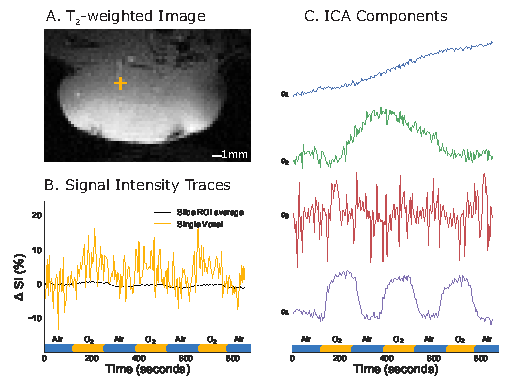
\includegraphics[width=0.5\textwidth]{oemri/oemri-images/fig1_technique.pdf} % requires the graphicx package
   \caption{(A) T$_2$W MRI of a tumor xenograft at 7T and (B) the corresponding T$_1$W signal-time traces of a single voxel (solid yellow) and whole-tumor slice ROI (dotted black) during gas cycling at two-minute intervals of air (x axis; blue) and O$_2$ (x axis;yellow).
(C) Plot of the four extracted ICA components from the entire tumor ROI, component \textbf{$c_4$} (purple) exhibits the same temporal features as the oxygen cycling time course shown along the bottom. All components are normalized, no vertical scale is shown.}
   \label{technique}
\end{figure}

\subsection{ICA enabled dOE-MRI detects variable oxygenation in a range of tumor models}
Tumors of human and murine origin and comprising a variety of tumor microenvironments were imaged, including fast growing, highly vascularized murine squamous cell (SCCVII) and human ovarian carcinomas (SKOV3), slower growing and well vascularized human breast cancer (BT-474), as well as a relatively fast growing but more poorly vascularized human colon colorectal carcinoma (HCT-116).
The inter-model heterogeneity of the tumors is reflected in the mean fraction of negative voxels in the dOE-MRI maps, which were 46 $\pm$ 6\% for BT-474, 36$\pm$3\% for HCT-116, 31$\pm$5\% for SCCVII, and 14$\pm$4\% for SKOV3 tumors. 
Considerable intra-tumor heterogeneity is also observed within some models, particularly the BT474.
dOE-MRI maps representing the mean fraction of negative voxels are shown for each tumor type in Figure~\ref{versatile}.
\begin{figure}[htbp]
   \centering
   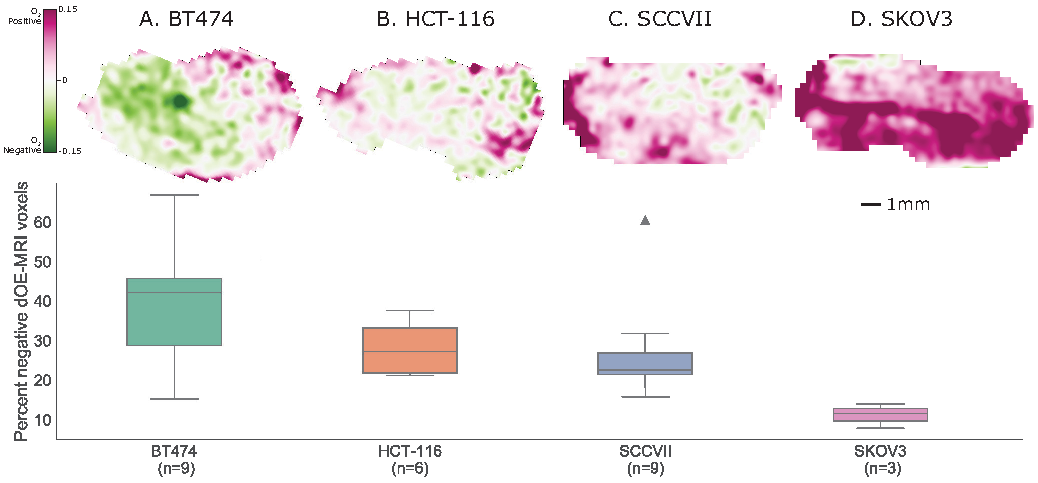
\includegraphics[width=\textwidth]{oemri/oemri-images/fig2_versatile.pdf} % requires the graphicx package
   \caption{Top: dOE-MRI maps for four tumor models HCT-116, BT-474, SCCVII, and SKOV3 are shown. Chosen slices are representative of the mean percent negative dOE-MRI fraction for the respective tumour model.
Bottom: The box-whisker plot shows the quartiles of percent negative dOE-MRI voxels for all imaged tumours.
\label{versatile}}
\end{figure}

\subsection{dOE-MRI with ICA does not require assumption of a response function}
To determine whether dOE-MRI maps obtained with a model-free ICA approach (Figure~\ref{fig_correlation}A) are comparable to maps assuming a mathematical model of the response, alternative oxygenation status maps were constructed. 
In Figure~\ref{fig_correlation}B and C, two example mathematical models - a square wave and the estimated hemodynamic response function (HDRF) - are correlated to the voxel-by-voxel raw time signal. 
Regions most correlated with the input paradigm remained purple in both alternative maps generated from modeled response functions.
Particularly when using the HDRF, the alternative oxygenation map showed very similar patterns in the regions demarcated as O$_2$-positive and O$_2$-negative. 
However, the map generated from correlating a square wave led to consistent underestimation of oxygenation relative to the model-free dOE-MRI map.

\begin{figure}[htbp]
   \centering
   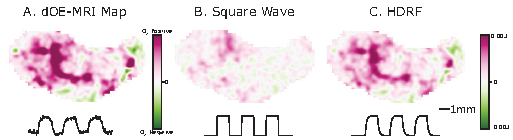
\includegraphics[width=\textwidth]{oemri/oemri-images/fig3_correlation.pdf} % requires the graphicx package
   \caption{(A) dOE-MRI map of an SCCVII tumor where purple voxels contribute strongly to the extracted component using ICA in the T$_1$W signal timecourses. 
Green voxels in the dOE-MRI map have a strong contribution of the inverse extracted component. Pearson's r-maps are shown correlating the raw time-signal voxel by voxel with a square wave (B), and an exponential convoluted with a square wave called the hemodynamic response function (HDRF) (C).
   \label{fig_correlation}}
\end{figure}
\subsection{Variability of response in individual oxygen cycles}

A full dOE-MRI sequence involved three cycles of oxygen but to assess the potential for shortening the sequence we also separately applied ICA to each of the three oxygen cycles independently.
Separate dOE-MRI maps, as well as voxel-wise correlation plots of a representative SCCVII tumor, are shown in Figure~\ref{fig_repeatability} with Pearson's r$_{all-1}$=0.74,r$_{all-2}$=0.86,r$_{all-3}$=0.84.
Pearson's r ranged from 0.79 to 0.87 for a similar analysis in a representative HCT-116 tumor.

The stability of the independent component extraction was assessed by undersampling the full timecourse threefold prior to application of ICA, and a high correlation between the dOE-MRI maps from full and three-fold undersampled timecourses is observed (Figure~\ref{fig_repeatability}E; Pearson's r = 0.84). 

\begin{figure}[htbp]
   \centering
   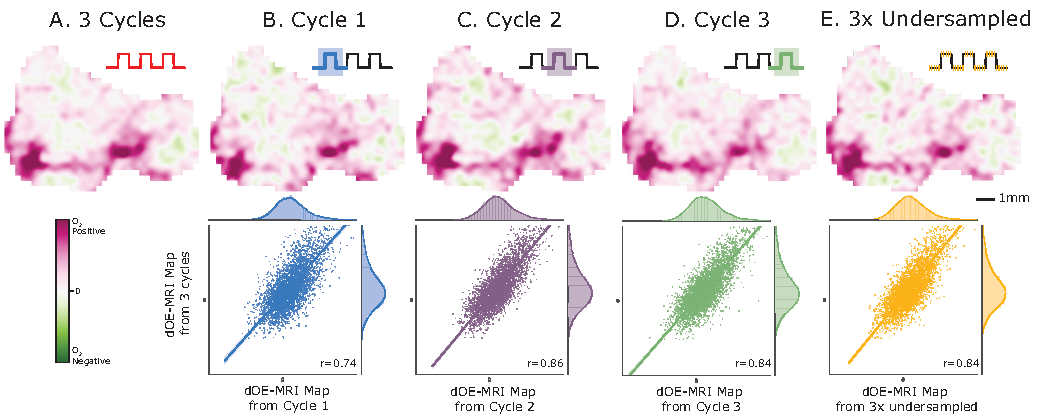
\includegraphics[width=\textwidth]{oemri/oemri-images/fig4_repeatability.pdf} % requires the graphicx package
   \caption{The dOE-MRI map including the full dataset of all three cycles (A) is compared to each of the three gas cycles separately (B,C,D), and to a map that temporally undersamples by selecting every third datapoint from the full dataset (E).
Voxel-wise plots of each map are correlated to the full dataset and a linear regression with Pearson's r is shown.
   \label{fig_repeatability}}
\end{figure}
\subsection{dOE-MRI maps correspond to matched histology sections}

Tumor tissue cryosections obtained to match MR imaging slices were stained for vasculature (CD31) and regions of pimonidazole-labeled hypoxia and are compared side-by-side; Figures~\ref{fig_sccvii} and~\ref{fig_hct116} provide five examples for each of SCCVII and HCT-116 tumor models for detailed review.
Generally, in corresponding dOE-MRI maps for both tumor models O$_2$-positive voxels align with the most oxygenated regions of histology sections, where pimonidazole labeling is absent, however many areas of mismatch are also observed. 
More consistent is that O$_2$-positive voxels do not typically correspond to tissues identified as hypoxic in the histology sections (i.e. labeled with pimonidazole).
In general, the more necrotic HCT-116 tumours have fewer oxygenated (O$_2$-positive) regions and significantly more hypoxic (O$_2$-negative) regions in the dOE-MRI maps, compared to the SCCVII tumors that have no necrosis. 
Pimonidazole labeling is heterogeneously dispersed within regions of viable tissue containing tumor blood vessels for both SCCVII tumors, Figure~\ref{fig_sccvii}, and HCT-116 tumors, which typically have greater amounts of necrosis, Figure~\ref{fig_hct116}.
Figure~\ref{histo_correlations} shows the fraction of negative dOE-MRI voxels correlated with the histological hypoxic fraction. 
For SCCVII tumours (n=9) there was an excellent correlation, with Pearson's r = 0.91 (\textit{p}=0.0016). 
However the correlation in the HCT-116 tumors (n=6) was poor, with r=0.13 (\textit{p}=0.81). 

\begin{figure}[htbp]
   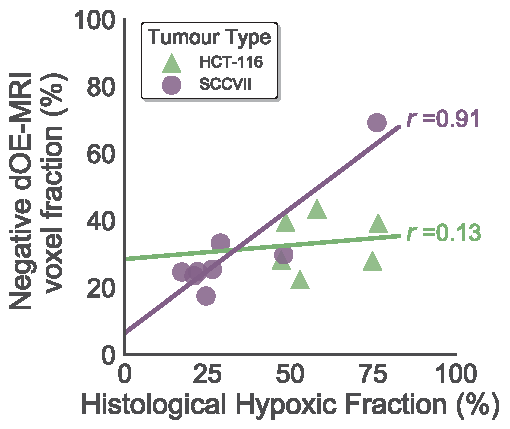
\includegraphics[width=0.5\textwidth]{oemri/oemri-images/fig5_histocorrelation.pdf} % requires the graphicx package
   \caption{The proportion of negative dOE-MRI voxels is plotted against the histological hypoxic fractions with Pearson's r = 0.91 for SCCVII tumours and r = 0.13 for HCT-116 tumours.
   \label{histo_correlations}}
\end{figure}

\begin{figure}[htbp]
   \centering
   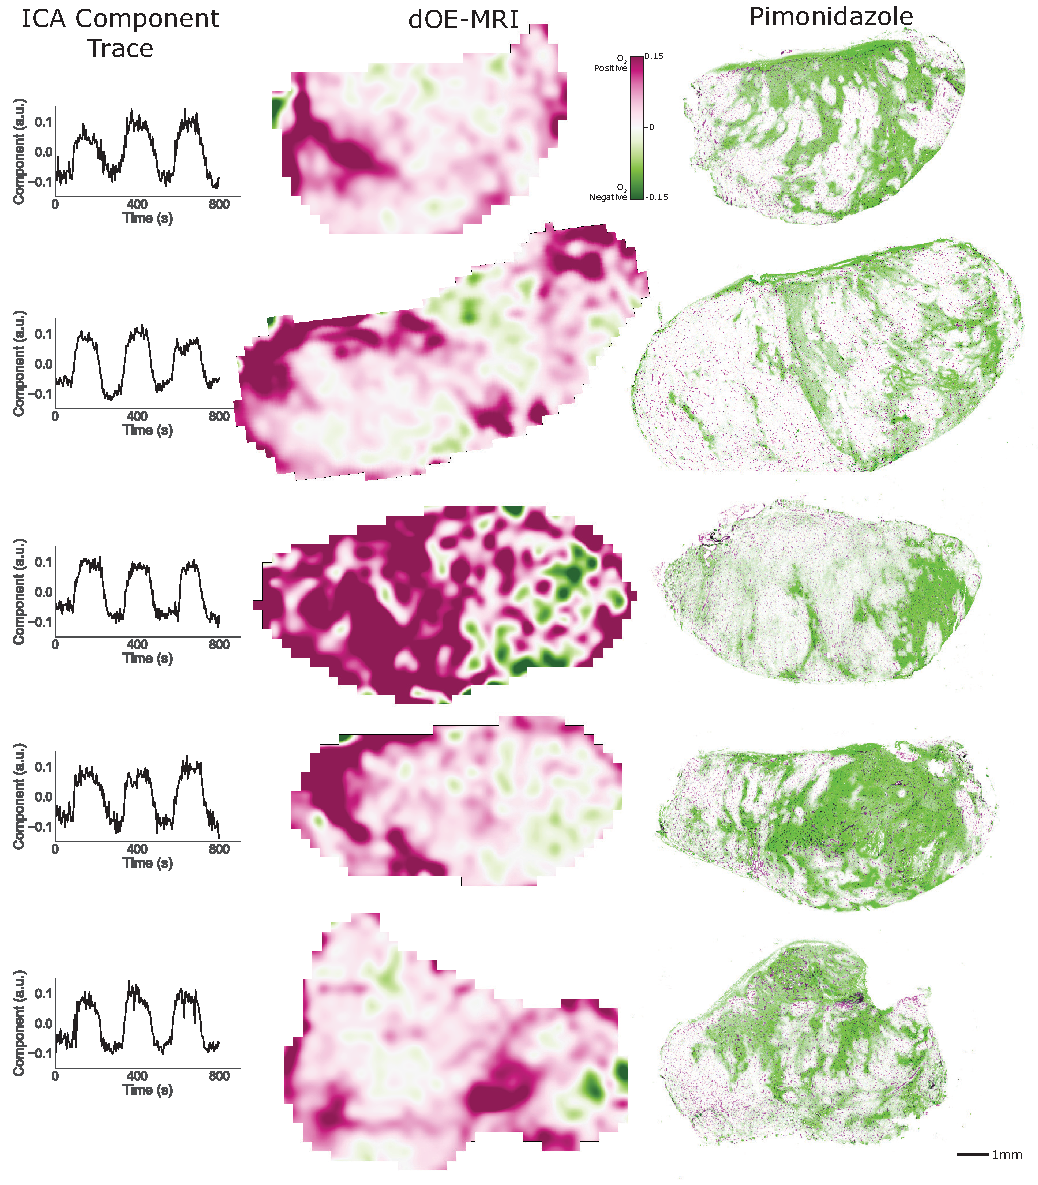
\includegraphics[width=0.9\textwidth]{oemri/oemri-images/fig6_sccvii.pdf} % requires the graphicx package
   \caption{SCCVII murine tumors with slice-matched histological images depicting pimonidazole-labeled hypoxia (green) and CD31-stained vasculature (purple) are shown next to the dOE-MRI parameter maps similarly colored with O$_2$-positive (purple) and O$_2$-negative (green) areas. Corresponding ICA extracted components are also shown.
   \label{fig_sccvii}}
\end{figure}
\begin{figure}[htbp]
   \centering
   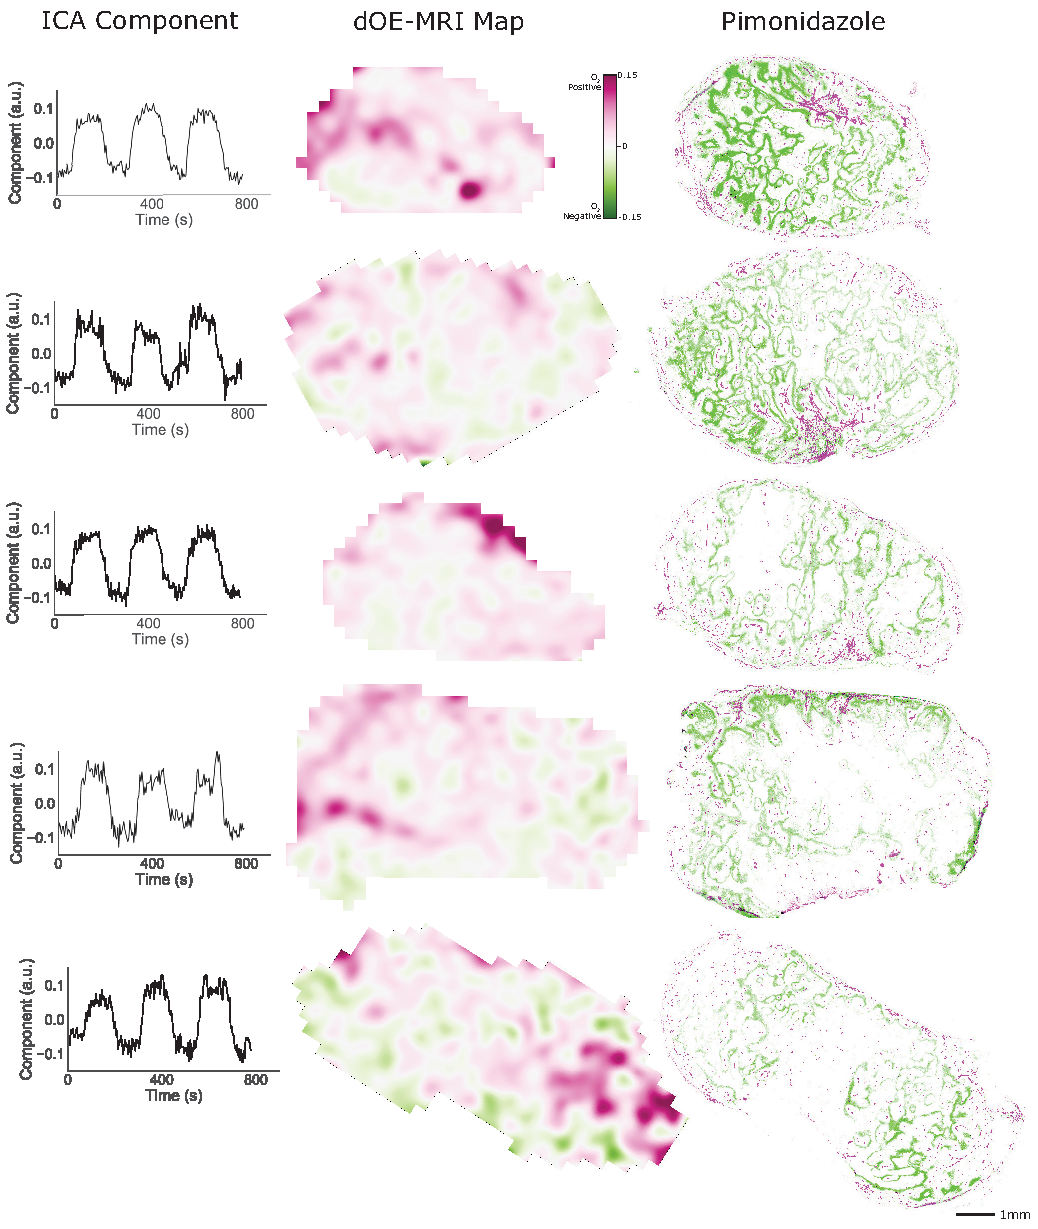
\includegraphics[width=0.9\textwidth]{oemri/oemri-images/fig7_hct116.pdf} % requires the graphicx package
   \caption{HCT-116 human colorectal xenografts with slice-matched histological images depicting pimonidazole-labeled hypoxia (green) and CD31-stained vasculature (purple) are shown next to the dOE-MRI parameter maps similarly colored with O$_2$-positive (purple) and O$_2$-negative (green) areas. Corresponding ICA extracted components are also shown.
   \label{fig_hct116}}
\end{figure}

%======================================================================
\section{Discussion}
% ======================================================================
Here we present an improved method for OE-MRI that employs two synergistic techniques to achieve higher speed and greater sensitivity.
First, a repeated gas challenge is used to probe tissue response by introducing an independent signal modulation unrelated to nuisance contributions such as temperature drifts and motion.
A repeating gas challenge improves the detection sensitivity of small amplitude signal changes that are typical of oxygen-enhanced MRI.
Second, a repeating signal modulation enables further improved sensitivity through the use of ICA, a signal processing technique to isolate source signals - T$_1$W changes due solely to the cycling oxygen - without knowledge of the tissue response (Figure~\ref{technique}).
While it is possible to generate correlation maps of the oxygen cycling paradigm with T$_1$W signal changes that appear very similar to dOE-MRI maps, an \emph{a-priori} assumption of a response function is required for this approach (Figure~\ref{fig_correlation}).
Furthermore, presupposing a particular oxygen response function biases the identification of responding O$_2$-positive voxels (Figure~\ref{fig_correlation}) underscoring the need for a model-free approach to extracting the oxygen-responding component.

The improved sensitivity of our technique results in broader applicability of dOE-MRI, as we found that an oxygen-enhancing component was extracted successfully in all imaged animals across a range of tumor models and environments (Figure~\ref{versatile}).
The unambiguous match of the identified component with the periods of the gas cycles increases the confidence that the small T$_1$W signal changes result from increased oxygen dissolved in the plasma and interstitial tissue fluids.
Maps from other extracted components (Supporting Information Figure S1) exhibit spatial patterns that could provide clues to the signal sources but associating meaning to them is challenging and would require additional data.
For example, even moderate shifts in temperature could drive a measurable change in T$_1$W signal during the timecourse, and a physiological monitoring system that is time-synced to the MR acquisition could illuminate this confounding variable. 
Nevertheless, we have established reliability of the technique by comparing maps from each cycle of the gas challenge to the map incorporating data from all three oxygen-cycles and have found no significant differences.
In fact, the strong correlations between dOE-MRI maps from each of the individual cycles of the gas challenge (Figure~\ref{fig_repeatability}) show that it is feasible to assess tissue oxygenation within 6 minutes.
Performing this analysis again with three-fold temporally under-sampled data suggests that there is sufficient SNR to successfully extract the oxygen responsive component (Figure~\ref{fig_repeatability}) with even a subset of the data. 

A limitation of OE-MRI is the difficulty in interpreting areas that do not show a reduction in T$_1$ as they may be either dead tissues that are \textit{unperfused and not oxygenated} or living, viable tissues that are \textit{perfused but not oxygenated} due to poor oxygen content of the supplying vessels. 
The latter population are of greater interest to the oncology community as it is these hypoxic but viable cells that have significant influence on treatment outcomes~\cite{Horsman:2016go}. 
The dOE-MRI technique presented here successfully correlates tumor oxygenation dOE-MRI and histology measures in SCCVII tumors but, despite improvements to sensitivity, a similar quantitative comparison in the HCT-116 tumor line showed poorer association (Fig.~\ref{histo_correlations}). 
This is likely attributable to the much higher amounts of necrosis typical of the HCT-116 model relative to SCCVII (Figs.~\ref{fig_sccvii} and \ref{fig_hct116}).
Mitigations to this limitation have been explored elsewhere and generally require a perfusion mask or $T_2^*$ - either technique can be added to the OE-MRI method proposed here to exclude necrosis and further improve sensitivity of the technique.

Application of existing OE-MRI techniques across a range of tumour models with varying perfusion characteristics has yielded mixed success without masking for perfused tissue.
For instance, O'Connor reported that in the highly perfused 786-0-R tumor lines, 85-96\% of all imaged tumor voxels were deemed to be oxygen-enhancing~\cite{OConnor:2016ee}.
In those tumors, there was a good correlation between histological hypoxic fraction and oxygen refractory voxels.
However, in the more weakly perfused SW620 tumors where only 76\% of the voxels are oxygen-enhancing, there were no significant correlations with the histological hypoxic fraction.
These issues were resolved by combining OE-MRI with DCE-MRI as a perfusion mask to select only perfused voxels for oxygenation assessment, thereby distinguishing between the viable hypoxic environment and necrotic dead tissues and improving the specificity and sensitivity of OE-MRI data. Using an IAUGC$_{60}$ map from DCE-MRI as a mask to obtain Oxy-R fractions O'Connor et al. showed good correlation with the histological hypoxic fraction~\cite{OConnor:2016ee}.
In more recent work, Little et al. showed oxygen enhancement in tumours with a histological hypoxic fraction as high as 43\%~\cite{Little:2018iu} and this translated very well to a study of six renal cell carcinoma patients.
Linnik et al. reported excellent correlation between percentage of ``negative AUC$_{OE}$'' ($O_2$-negative) voxels and percentage of hypoxic areas in the highly vascular preclinical U87MG tumor xenografts~\cite{Linnik:2013hf}.
A second approach for differentiating between viable but hypoxic regions and unperfused dead tissues, is to combine OE-MRI with $T_2^*$W acquisition and the BOLD effect to classify regions~\cite{Little:2018iu,Zhao:2015ez,White:2016fz,Burrell:2013je,Yang:2018vo} that show both effects. 
Excess oxygen in the blood will induce changes in Hb saturation, which alter the T2* resulting in a robust measure of areas with functioning vasculature. 
Conceivably, the saved acquisition time achieved with under-sampling T$_1$W dOE-MRI suggests that $T_2^*$W images could also be acquired to concurrently assess the blood oxygen level dependent (BOLD) response. 

Within the relatively short 14-minute imaging time, both the HCT-116 and SCCVII tumours show only minor changes in the oxygenation maps between cycles (Figure~\ref{fig_correlation}).
In longer imaging sessions, or during administration of an intervention, these same tumors may exhibit varying oxygenation patterns between cycles.
Periods of oxygen-starvation and re-oxygenation in tumors have been termed intermittent hypoxia and can arise due to temporary vessel occlusions~\cite{Dewhirst:2009de,Bayer:2011js}.
Recent work on measuring intermittent hypoxia in patients using R$_2^*$~\cite{Panek:2017ge} shows that interest in this phenomenon continues but the importance of intermittent hypoxia in tumors is unclear largely due to poor availability of techniques to measure it in the clinic~\cite{Michiels:2016hv}.
The relatively short imaging time for dOE-MRI makes assessing temporal oxygenation changes possible within a timescale on the order of minutes by comparing correlation maps generated from sequential cycles.

dOE-MRI offers a versatile technique where the duration of the cycles and gas challenge, temporal resolution and desired signal-to-noise can be modified based on the imaging objectives, which could include investigating intermittent perfusion or intervention-mediated changes in the tumor microenvironment. 
Of note, supplying excess oxygen to hypoxic tumor cells over time has the potential for increasing the baseline oxygen concentration, effectively reducing the hypoxic fraction and altering the tumor microenvironment~\cite{Linnik:2013hf}.
This would result in voxels becoming more oxygen responsive over progressive oxygen cycles and would depend on the tumor characteristics as well as the duration of the oxygen challenge.
This was not observed on the time scales in our study when using ICA to extract changes in T$_1$W signal intensity just due to the gas challenge. 
Should it arise in other contexts it could possibly be mitigated by extending the air-breathing part of the cycle, or by extracting that as a separate component using ICA.
The potential for creating a hyperoxia steady state by modulating oxygen duration is discussed further by Losert et al ~\cite{Losert:2002gt}.

Typically, histological validation of MR data is done by collapsing rich histology data into a single metric, such as a hypoxic fraction, with whole-tumor or single-slice average comparisons.
While this is sometimes a useful validation approach, it may not reflect the highly heterogeneous patterns of hypoxia that are known to vary spatially and temporally, even within the same tumor, as well as between tumor types as highlighted in Figures~\ref{histo_correlations}-\ref{fig_hct116}. 
Further complications are encountered with respect to validation of tools to assess hypoxia considering that hypoxia is not simply a binary metric. Instead, tumor oxygenation exists as a spectrum beginning with some tissues that may be normoxic, at levels similar to neighboring normal tissues of origin, and can continue decreasing through levels of hypoxia to near anoxia where cells are still viable but are no longer able to proliferate.
Eventually cells die in the absence of oxygen, and when this occurs in large numbers there can be significant regions of necrosis in solid tumors. 
A range of oxygenation levels are likely to be present in the highly heterogeneous microenvironments of all solid tumors, but what is of interest to the oncology community is \emph{clinically relevant} hypoxia~\cite{Horsman:2012kw}.
This refers to measurable tumor oxygenation levels that are biomarkers of physiologically meaningful phenomena, including patient prognosis or tumor sensitivity to treatments, such as immunotherapy or radiotherapy. The relevant oxygenation status for any biomarker of interest may include levels spanning from moderate to severely hypoxic. 
Pimonidazole has been demonstrated as a clinically relevant marker of hypoxia, but poor or inconsistent correlation with pimonidazole, as we have seen in our imaged tumors, does not exclude other measures of tumor oxygenation from potential utility.

Measurable pimonidazole-adduct formation occurs when the O$_2$ tension in the vicinity drops below 10 mmHg~\cite{Gross:1995wq} but in dOE-MRI, O$_2$-positive voxels are extracted as excess oxygen dissolves in the plasma and interstitial tissue fluid to decrease T$_1$.
Voxels where T$_1$ has significantly increased has previously been correlated to poorly perfused regions and likely corresponds to hypoxic regions where the excess oxygen is picked up by deoxyhemoglobin molecules~\cite{Linnik:2013hf,Burrell:2013je,Remmele:2012df}.
The exact mechanism for a T$_1$ increase as a result of oxygen inhalation has not yet been confirmed~\cite{Zhao:2015ez,Linnik:2013hf}, however, based on careful work of Silvennonin et al., characterizing behavior of T$_1$ in fresh bovine blood~\cite{Silvennoinen:2003gn}, we speculate the corresponding T$_1$W signal decrease may arise due to the conversion of deoxyhemoglobin to hemoglobin in the perfused vessels of hypoxic regions .
O$_2$-positive regions in dOE-MRI maps are generally in good agreement with well perfused areas of histology images for both HCT-116 and SCCVII tumors, as shown in Figures~\ref{fig_sccvii} and~\ref{fig_hct116}.
Voxels exhibiting signal reduction with the O$_2$ stimulus in dOE-MRI maps (O$_2$-negative, green) typically correspond with histology (pimonidazole, green) but not all pimonidazole-labeled regions appear as O$_2$-negative voxels.
Similarly, CD31-stained tumour regions are not exclusively O$_2$-positive in the dOE-MRI maps because not all tumor vessels are perfused.
In fact many perfused blood vessels are only intermittently perfused and consequently, the measurement of hypoxia is time-sensitive.
Mismatches between dOE-MRI and histology may be attributed in part to the different sensitivities and detection thresholds for measuring hypoxia and oxygenation in the dOE-MRI and histology-based modalities, as well as potential mismatch between the timing of pimonidazole-labeling and dOE-MRI data acquisition . 

Depending on the application of dOE-MRI, quantitative O$_2$-positive and O$_2$-negative fractions can be obtained from dOE-MRI maps as shown in this study, by deploying group ICA techniques~\cite{Calhoun:2009jr}, or setting significance thresholds using a t-test~\cite{Greicius:2004ck} and computing z-scores~\cite{McKeown:1998wd}.
To help understand the oxygen dynamics in tumors, including the effect of hemoglobin with T$_2^*$ mapping, fitting exponential recovery and decay curves to the extracted oxygen response curves may provide additional insights as originally proposed by Losert et al. in the brain~\cite{Losert:2002gt}.
In a promising study, White et al. has shown that OE-MRI may be very relevant in developing prognostic factors to predict tumor response to hypofractionation by stratifying tumors that may benefit from oxygen breathing during irradiation~\cite{White:2016fz}.
Featherstone et al. have recently explored pre-clinical datasets using feature-extraction and clustering analysis and this may prove fruitful in understanding the behavior of subregions within a tumour microenvironment~\cite{Featherstone:2018cn}.
Future work to evaluate the utility of dOE-MRI will ultimately depend on its context-dependent validation as a relevant measure of tumor hypoxia to dynamically characterize the clinically relevant oxygen status of tumors, relating this information to treatment sensitivities and outcomes.

\begin{figure}[htbp]
   \centering
   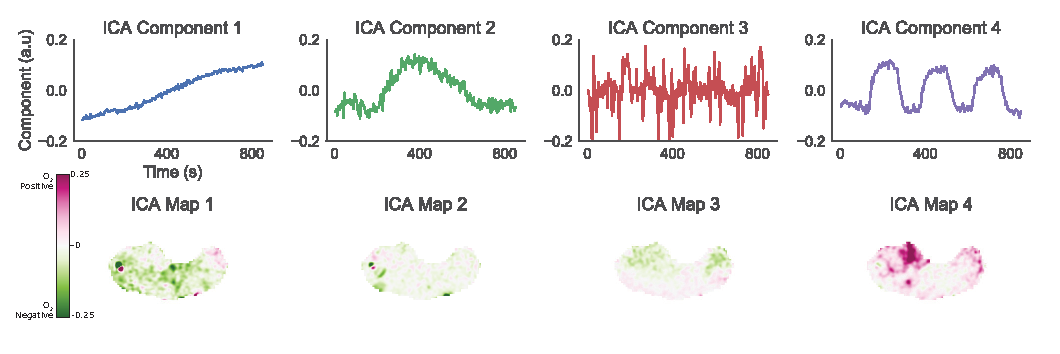
\includegraphics[width=0.9\textwidth]{oemri/oemri-images/fig_components.pdf} % requires the graphicx package
   \caption{Plots of the four components extracted from ICA are shown (($||c_i||=1, \forall i $) along with the corresponding  weighting factor maps (normalized to mean voxel wise mean signal intensity). Note that c$_4$ is clearly the component of interest here as the cycling pattern is not present in any other component. We speculate that c$_1$ corresponds to a temperature drift over the course of the scan and c$_3$ is likely related to a breathing motion artefact. Component 2 is a relatively weak spurious signal fairly low in magnitude with no obvious spatial or temporal pattern. Further investigation is required to explore the underlying physiological response (if any) of the other components.
   \label{Sfig_components}}
\end{figure}



% ======================================================================
\section{Conclusions}
% ======================================================================
In this study we extend existing oxygen-enhanced MRI techniques by adding a cycling element to the respiratory challenge and using a blind-source separation signal processing technique (ICA) to extract the oxygen responsive component and responding voxels.
This dOE-MRI method presents significant improvements to the sensitivity and applicability of OE-MRI where small changes in T$_1$W signal intensity arising from cycling respiratory challenges can be separated robustly. Traditional quantitative T$_1$ mapping techniques have longer imaging times and are impractical for OE-MRI due to SNR and time constraints.
dOE-MRI with ICA is clinically translatable as the sequence acquisition is relatively short and most centers already have access to dynamic T$_1$W MRI acquisitions that many patients already routinely receive. 
Therefore dOE-MRI is an exciting, non-invasive and widely available technique for assessing tumor oxygenation that could provide a crucial tool in the field of radiation oncology and in the development of treatments targeting the tumor microenvironment.

% ======================================================================
\section{Acknowledgments}
% ======================================================================

Dr. Martin McKeown provided assistance in understanding the utility of ICA in the given context. Dr. Alastair Kyle undertook foundational work by designing and building the microscope and histology acquisition system. 


\endinput

\section{Supporting Information}

Additional Supporting Information may be found in the online version of this article.

\textbf{Supporting Information Figure S1}. Plots of the four components extracted from ICA are shown (($||c_i||=1, \forall i $) along with the corresponding  weighting factor maps (normalized to mean voxel wise mean signal intensity). Note that c$_4$ is clearly the component of interest here as the cycling pattern is not present in any other component. We speculate that c$_1$ corresponds to a temperature drift over the course of the scan and c$_3$ is likely related to a breathing motion artefact. Component 2 is a relatively weak spurious signal fairly low in magnitude with no obvious spatial or temporal pattern. Further investigation is required to explore the underlying physiological response (if any) of the other components.
